\chapter{Framework}
\label{ch:methode}

In Kapitel \ref{ch:theorie} wurde das theoretisch-mathematische Modell beschrieben, mit welchem ein Bit geschrieben und wieder rekonstruiert werden kann. Um dieses Wissen nun praktisch nutzen zu können wurde ein Framework ausgearbeitet in dem es zur Anwendung kommt. 

\section{Architektur}

Das von Shannon und Weaver entwickelte Sender-Empfänger-Modell \cite{shannon2001mathematical} kann herangezogen werden, um den Aufbau des Frameworks zu modellieren:

\begin{figure}[tb]
	\centering
	%\includesvg[width=0.7\textwidth]{figures/diagram-framework.svg}
	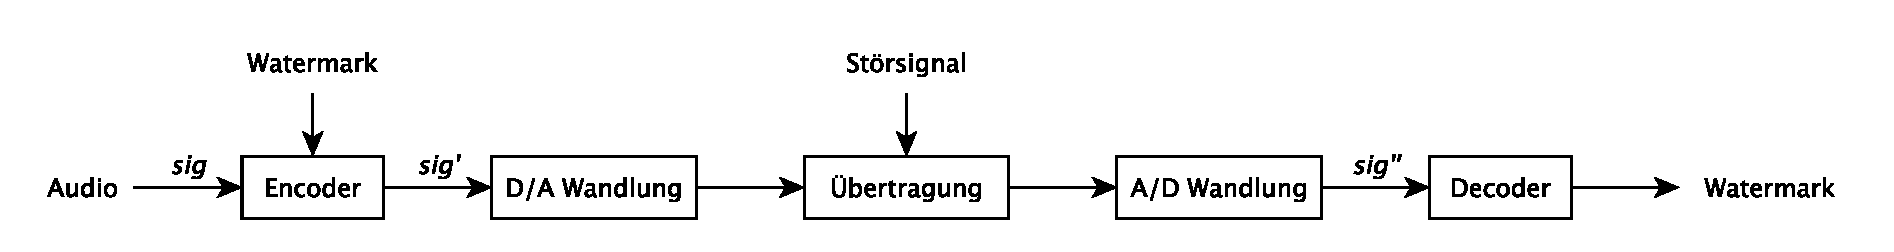
\includegraphics[width=0.9\textwidth]{figures/diagram-framework.pdf}
	\caption{Schematischer Aufbau des Frameworks}
	\label{fig:diagram-framework}
\end{figure}

An dieser Stelle ist der Zusammenhang der Module zu den mathematischen Grundlagen gut ersichtlich:

\begin{description}

\item[Encoder] \index{Encoder}
Dieses Modul nimmt ein digitales Signal und reichtert es mit zusätzlicher Information (dem Watermark) an. Das Ergebnis ist erneut ein digitales Signal, welches als \textit{wav} File vorliegt. Dies geschieht durch die in Abschnitt \ref{sec:embeddingstragety_bitsequence} beschriebene Methode. 
\item[D/A Wandlung] \index{Encoder}
Die Digital-Analog Wandlung wird das digitale Signal (also das wav-File) in ein analoges umgewandelt. In der Regel geschieht dies durch Lautsprecher, die ein elekrtisches Signal in Schallwellen umwandeln. Das Signal wird hier also für den Menschen hörbar. 
Eine D/A Wandlung geschieht aber auch, wenn die digitalen Daten in ein elektrisches (analoges) Signal umgewandelt werden, etwa wie es am Line-out Ausgang einer Soundkarte anliegt. 
\item[Übertragung] \index{Übertragungskanal}
Die Übertragungs 


	
\end{description}

\section{Watermark Implantierung}
\label{sec:embedding}

\begin{figure}[tb]
	\centering
	%\includesvg[width=0.7\textwidth]{figures/diagram-framework.svg}
	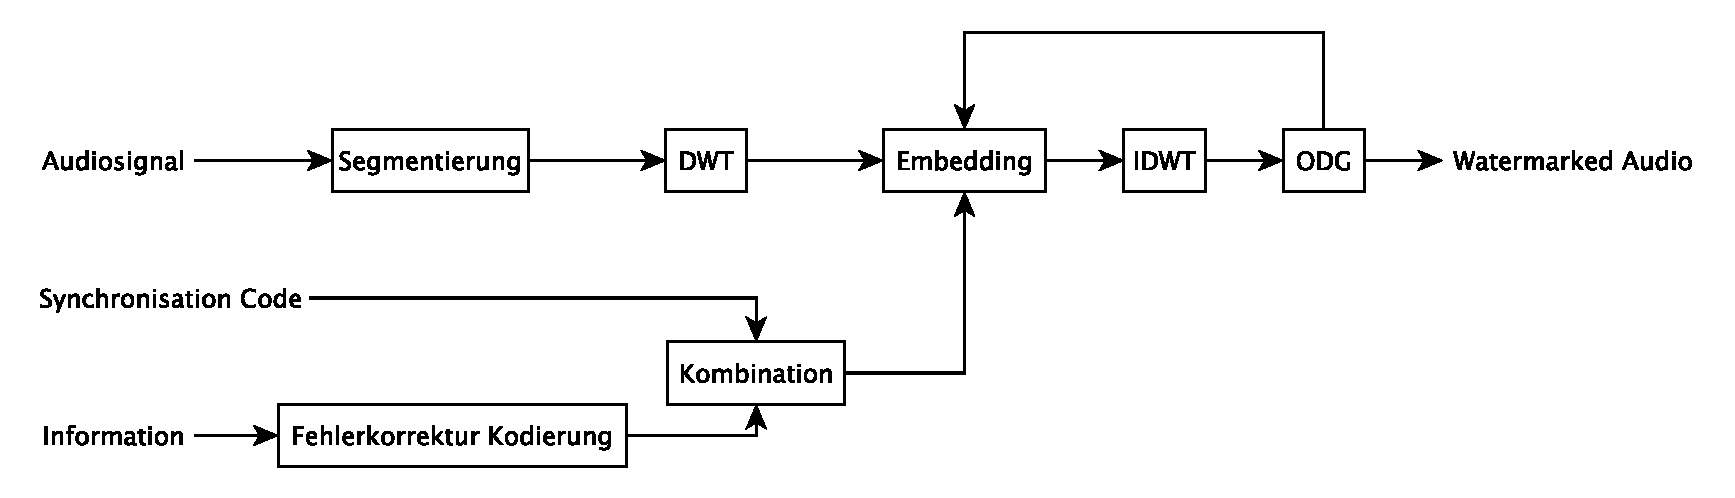
\includegraphics[width=0.9\textwidth]{figures/diagram-encoder.pdf}
	\caption{Schematischer Aufbau des Implemetierungsprozesses}
	\label{fig:diagram-encoder}
\end{figure}

\subsection{Synchronisations-Codes}

wozu sync codes ganz allgemein

\subsection{Fehlerkorrekturverfahren}
\label{sec:errorcorrection}

Error detection and correction


Wir verwenden hier Vorwärtsfehlerkorrektur \index{Vorwärtsfehlerkorrektur} (in der englischen Literator \textit{forward error correction} \index{forward error correction|see{Vorwärtsfehlerkorrektur}}, daher kurz FEC) beidem die Daten mit einem \textit{error-correcting code} \index{error-correcting code} (ECC) mit redundanten Daten angereichert werden.

\subsubsection{BCH-Codes}

\cite{chang2012location} \cite{huang2002blind}

\subsubsection{RS-Codes}

\subsubsection{Turbo-Codes}

\subsubsection{LDPC-Codes}

\subsection{Datenstrukturen und Protokoll}
\label{sec:protokoll}

\subsection{Qualitätskontrolle und ODG }
\label{sec:qualitaetskontrolle}

\subsubsection{Mean Opinion Score (MOS)}

\cite{??}

\subsubsection{Signal-Rauschabstand (SNR)} \index{Signal-Rauschabstand}

\subsubsection{Objective Difference Grade (ODG)} \index{Objective Difference Grade}

Eine kleine Evaluierung gängiger PEAQ Implementierungen findet sich in Anhang \ref{ch:peaq}.


\section{Watermark Extrahierung}
\label{sec:extraction}

\begin{figure}[tb]
	\centering
	%\includesvg[width=0.7\textwidth]{figures/diagram-framework.svg}
	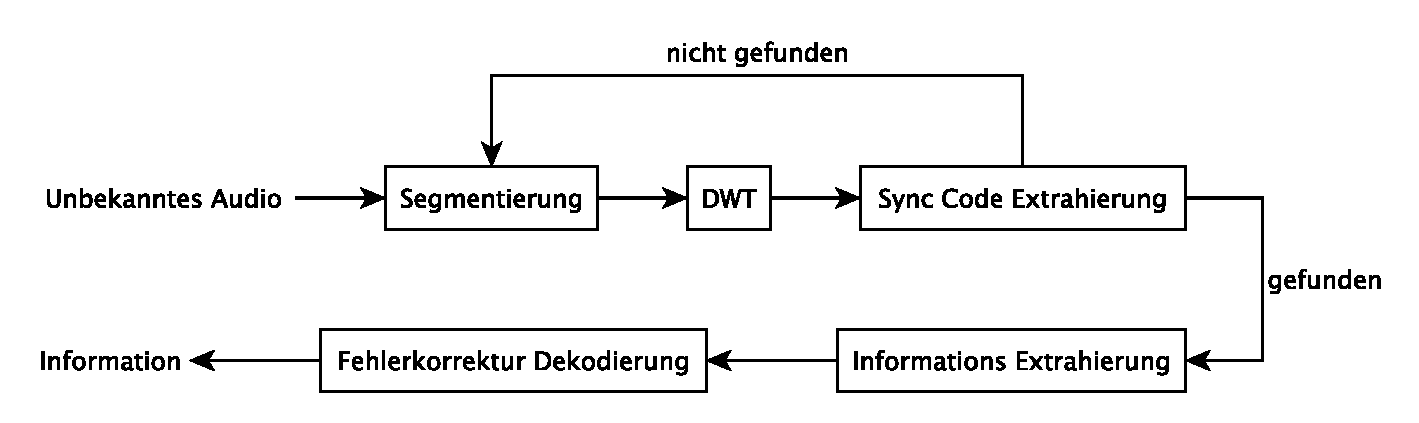
\includegraphics[width=0.9\textwidth]{figures/diagram-decoder.pdf}
	\caption{Schematischer Aufbau des Extraktionsprozesses}
	\label{fig:diagram-decoder}
\end{figure}

\subsection{Resynchronisaton und Interpolation}

\subsection{Synchronisations-Code Erkennung}

\subsubsection{Autokorrelation und Barker-Codes} \index{Barker-Code}
\label{sec:barkercode}


vorteil der barker codes, autocorrelation

\subsection{Datenextrahierung}



